\section{Conditional Optical Service Certificate}
\subsection{Reference-relative identity and angular geometry}
Let $e_0=q(t_0)+b$ and $d_i=q(t_0+s_i)-q(t_0)$. For fixed $b,\alpha$ and positive starting power, the exact identity is
\begin{equation}
\log\frac{p(t_0+s_i)}{p(t_0)}=
\log\frac{g(t_0+s_i)}{g(t_0)}-
\frac{2}{\alpha^2}\left(2e_0^Td_i+\norm{d_i}^2\right).
\label{eq:identity}
\end{equation}
The cross term retains the true starting angular error. Omitting it, or replacing delivered motion by commanded motion without an enclosure, can overstate the available margin.

\begin{proposition}[Angular loss over two balls]
Suppose $e_0\in\mathcal B(c,R)$ and $d_i\in\mathcal B(\bar d_i,r_i)$ with nonnegative Euclidean radii. Then $2e_0^Td_i+\norm{d_i}^2\leq\overline D_i$, where
\begin{align}
\overline D_i={}&2c^T\bar d_i+2R\norm{\bar d_i}+\norm{\bar d_i}^2\nonumber\\
&+2(\norm{c+\bar d_i}+R)r_i+r_i^2.
\label{eq:Dgeneral}
\end{align}
For $c=0$, the exact maximum is
\begin{equation}
D_{\max,i}=2R(\norm{\bar d_i}+r_i)+(\norm{\bar d_i}+r_i)^2.
\label{eq:Dcenter}
\end{equation}
\end{proposition}
\emph{Proof:} Write $e_0=c+u$, $d_i=\bar d_i+w$, $A=\norm{\bar d_i}$, $C=\norm{c+\bar d_i}$. Exact expansion gives
\begin{align}
\overline D_i-(2e_0^Td_i+\norm{d_i}^2)
={}&2(RA-u^T\bar d_i)\nonumber\\
&+2(r_iC-(c+\bar d_i)^Tw)\nonumber\\
&+2(Rr_i-u^Tw)+(r_i^2-\norm w^2).
\end{align}
Each summand is nonnegative by Cauchy--Schwarz, $\norm u\leq R$ and $\norm w\leq r_i$. For $c=0$, $A>0$, the choice $u=R\bar d_i/A$, $w=r_i\bar d_i/A$ attains \eqref{eq:Dcenter}. If $A=0$, use $u=Rz$, $w=r_i z$ for any unit vector $z$. These constructions include either radius zero and the singleton cases. Noncentered sharpness is not asserted.\hfill$\square$

All terms in $\overline D_i$ have dimension rad$^2$. Combining \eqref{eq:identity} with A1--A2 and $p(t_0)\geq\underline p_0$ gives
\begin{equation}
\underline p_i=\underline p_0\exp\left[-\ell s_i-
\frac{2\max(\overline D_i,0)}{\alpha_-^2}\right].
\label{eq:lower}
\end{equation}
For nonnegative angular loss, the smallest allowed divergence is conservative. If its upper bound is negative, replacing it by zero discards guaranteed improvement and avoids reversing the divergence inequality. Sharpness of the centered angular geometry does not imply tightness of \eqref{eq:lower}: optical priors, initial-power intervals and actuator uncertainty can be mutually coupled and conservatively separated.

\subsection{Simultaneous sensor event and numeric calibration}
Define the mission event
\begin{equation}
\mathcal E=\{ |Z_{k,j}|\leq\kappa\quad\text{for all }0\leq k<N,\ 1\leq j\leq5\}.
\end{equation}
With standard Gaussian marginal tails,
\begin{align}
\kappa&=\Phi^{-1}\!\left(1-\frac{\delta}{10N}\right),\nonumber\\
\Pr(\mathcal E^c)&\leq\sum_{k,j}\Pr(|Z_{k,j}|>\kappa)\leq\delta.
\label{eq:event}
\end{align}
The exact implementation uses $\sqrt2\operatorname{erfc}^{-1}[\delta/(5N)]$. Here $\delta=0.01$, $N=700$ for samples $0,.02,\ldots,13.98$~s, and $\kappa=4.680831082738$ (rounded). Each two-sided scalar tail is $\delta/(5N)=2.857142857\times10^{-6}$. This is a mission event, not a separate 99\% interval at each measurement. No independence assumption enters the union bound.

For $\eta=\kappa\sigma_p<1$, on $\mathcal E$,
\begin{equation}
\underline p_0=\frac{p_m(t_0)}{1+\eta}\leq p(t_0)\leq
\frac{p_m(t_0)}{1-\eta}=\overline p_0.
\label{eq:interval}
\end{equation}
The interval holds simultaneously at every index, hence also at an observation-selected trigger $\tau$. In particular,
\begin{equation}
\{\overline p_\tau<p_{\min}\leq p_\tau\}\subseteq\mathcal E^c.
\label{eq:falseenable}
\end{equation}
This avoids optional-selection misuse of a pointwise interval; it does not imply an exact coverage probability conditional on having triggered or accepted a fit.

An acquisition budget is enabled only when $\overline p_0<p_{\min}$. A straddling interval keeps the working-link budget. On $\mathcal E$ with positive power and $\eta<1$, the multiplier in \eqref{eq:sensors} is positive, so zero clipping is inactive. At true zero power, $p_m=0$ and the detector-floor rule refuses a probe. If $\eta\geq1$, the upper endpoint is unbounded and cannot enable acquisition.

\subsection{Starting-error enclosure and service theorem}
The source selector uses a centered enclosure. On $\mathcal E$, $\epsilon_q=\sqrt2\kappa\sigma_q$ bounds the encoder-vector error. Combining the offset prior with the measured angle gives $R_{\rm prior}=b_{\max}+\norm{q_m(t_0)}+\epsilon_q$. The optical identity at the start gives a second valid radius,
\begin{equation}
R_{\rm power}=\alpha_+\sqrt{\frac12\max\!\left\{0,\log\frac{p_{0,+}g_{\max}}{\underline p_0}\right\}},
\end{equation}
where $p_{0,+}$ is the maximum aligned power over the declared divergence interval. Thus $R=\min(R_{\rm prior},R_{\rm power})$ is valid whenever both priors are consistent. The positive-part operator is the implementation's conservative nonnegative convention; a physically inconsistent empty prior must not be treated as a new calibrated state estimate.

\begin{theorem}[Conditional sampled probe service]
Consider a candidate starting at a possibly observation-selected sample $\tau$ and ending within the $N$-sample mission. Suppose A1--A5 hold, the starting-error ball is valid, and for each window sample the delivered increment is contained in $\mathcal B(\bar d_i,r_i)$. On $\mathcal E$, let $\underline p_i$ be \eqref{eq:lower} using \eqref{eq:interval} and Proposition~1. Then $p_{\tau+i}\geq\underline p_i$. If the selector admits only candidates satisfying
\begin{equation}
\widehat O=h\sum_{i=0}^{H-1}\mathbf1\{\underline p_i<p_{\min}\}\leq B,
\end{equation}
the actual sampled probe-window outage is at most $B$. For otherwise valid contracts, any failure of this implication due to the stipulated sensor event is contained in $\mathcal E^c$, with unconditional mission probability at most $\delta$.
\end{theorem}
\emph{Proof:} On $\mathcal E$, the starting-power and error enclosures hold at every possible start. Proposition~1 bounds the angular-loss term at each candidate sample. A1--A2 then turn \eqref{eq:identity} into \eqref{eq:lower}. Pointwise, $\mathbf1\{p_{\tau+i}<p_{\min}\}\leq\mathbf1\{\underline p_i<p_{\min}\}$. Multiplying by $h$ and summing proves the outage implication. Simultaneity permits the selected start, and \eqref{eq:event} bounds its event-complement probability.\hfill$\square$

\emph{What the theorem does not prove:} It is not a continuous-time intersample guarantee, a formally rounded floating-point enclosure, a probability conditional on estimator acceptance, or a certificate of correct diagnosis. It establishes neither actual hardware calibration nor recovery after a later correction. Wrong tails, bias, continuous actuator parameters outside the finite set, or an offset changing within the window invalidate its premises. Figure~\ref{fig:geometry} illustrates the actual recorded quantities, not a new experiment.

\begin{figure*}[t]
\centering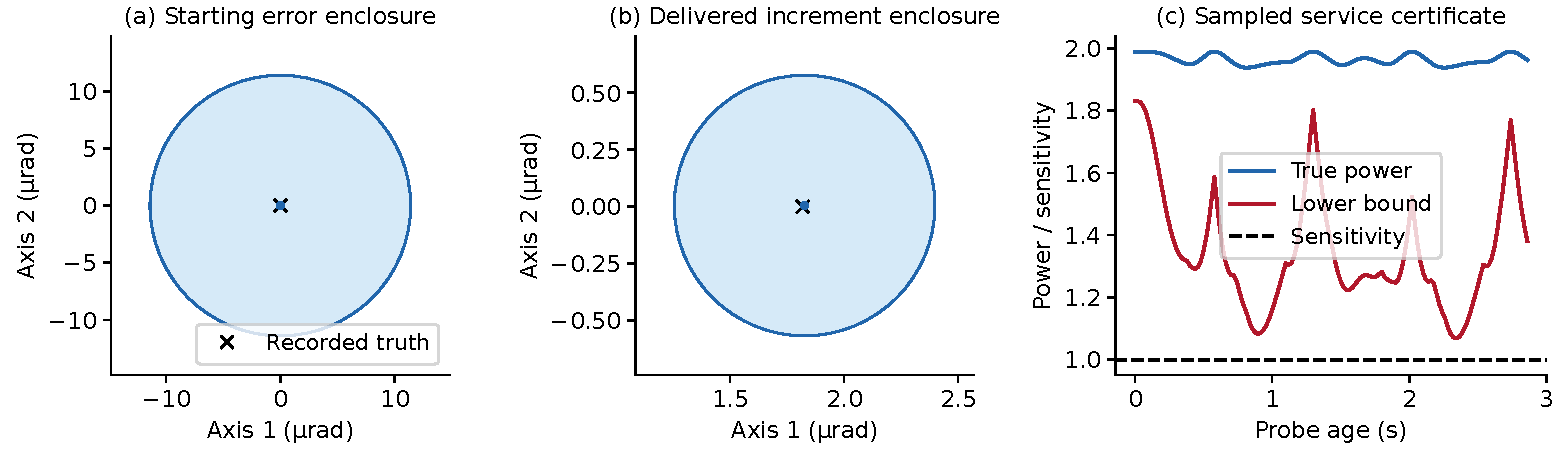
\includegraphics[width=\textwidth]{certificate_geometry.pdf}
\caption{Certificate geometry and actual power for region~1 midpoint, seed~7001, nominal actual actuator. The initial-error ball and one delivered-increment ball are in different coordinate planes; crosses show recorded truth. Panel (b) uses the middle probe sample. Panel (c) shows true and bounded power over the same recorded probe. Centers/radii are exported in the supplementary figure-source record.}
\label{fig:geometry}
\end{figure*}
